\documentclass[a4paper]{article}
\usepackage[utf8]{inputenc}
\usepackage{amsmath}
\usepackage[colorinlistoftodos]{todonotes}
\usepackage[utf8]{inputenc}
\usepackage{graphicx}
\graphicspath{ {figures/} }
\usepackage{array}
\usepackage{placeins}
\usepackage[margin = 0.5in]{geometry}
\PassOptionsToPackage{hyphens}{url}
\usepackage{hyperref}
\usepackage{parskip}
\usepackage [english]{babel}
\usepackage [autostyle, english = american]{csquotes}
\MakeOuterQuote{"}
\hypersetup{
     colorlinks,
     urlcolor    = blue
}
\usepackage{xcolor}
\usepackage{listings}
\lstloadlanguages{Python}
\newcommand{\inlinecode}[1]{\lstinline{#1}}

\lstset{
  language=Python,
  basicstyle=\scriptsize\sffamily,
  numberstyle=\color{gray},
  stringstyle=\color[HTML]{933797},
  commentstyle=\color[HTML]{228B22}\sffamily,
  emph={[2]from,import,pass,return}, emphstyle={[2]\color[HTML]{DD52F0}},
  emph={[3]range}, emphstyle={[3]\color[HTML]{D17032}},
  emph={[4]for,in,def}, emphstyle={[4]\color{blue}},
  showstringspaces=false,
  breaklines=true,
  prebreak=\mbox{{\color{gray}\tiny$\searrow$}},
  numbers=left,
  xleftmargin=15pt
}

\title{Application 4: Applications to Genomics and Beyond\\Algorithmic Thinking (Part2)}
\author{Shamsuddin Rehmani}
\begin{document}
\sloppy
\maketitle
\section*{Application 4 Description}
In Project 4, you implemented dynamic programming algorithms for determining both global and local alignments of pairs of sequences. In this Application, we will demonstrate the utility of these algorithms in two domains. In the first part of the Application, we examine an interesting problem from genomics. (This is based on "Introduction to Computational Genomics", by Nello Cristianini and Matthew W. Hahn). We will compare two sequences that have diverged from a common ancestor sequence due to mutation. (Mutation here includes base-pair substitution, which changes the sequence content, and insertion/deletion, which change the sequence lengths.) In the second part of the Application, we consider words that have spelling mistakes.

\noindent For the genomics part of the Application, you will load several protein sequences and an appropriate scoring matrix. For the spelling correction part of the Application, you will load a provided word list. To simplify these tasks, you are welcome to use this \href{http://www.codeskulptor.org/#alg_application4_provided.py}{provided code}.

\section*{Comparing two proteins}
In 1994, Walter Gehring and colleagues at the University of Basel carried out an "interesting" experiment: they were able to turn on a gene called eyeless in various places on the body of the fruit fly,Drosophila melanogaster. The result was astonishing - fruit flies developed that had whole eyes sprouting up all over their bodies. It turned out that the eyeless is a master regulatory gene - it controls a cascade that contains more than 2000 other genes. Turning it on anywhere in the body activates the cascade and produces a fully formed, but non-functioning, eye. Humans, as well as many other animals, have a slightly different version of the eyeless gene (that is, a similar, yet not identical sequence of the same gene).

This observation suggests that about 600 million years ago (the estimated time of divergence between humans and fruit flies) there was an ancestral organism that itself used some version of eyeless, and that throughout the evolution of humans and fruit flies this gene continued to be maintained, albeit while accumulating mutations that did not greatly affect its function. In particular, a substring of the eyeless protein of about 130 amino acids, known as the PAX domain, whose function is to bind specific sequences of DNA, is virtually identical between the human and fruit fly versions of eyeless.

In following questions, we compute the similarity between the human and fruit fly versions of the eyeless protein and see if we can identify the PAX domain.

\section*{Answer to Question 1}
Score of local Alignment = 875

Local alignment of HumanEyelessProtein:

\textit{HSGVNQLGGVFVNGRPLPDSTRQKIVELAHSGARPCDISRILQVSNGCVSKILGRYYETGSIRPRAIGGSK\\
PRVATPEVVSKIAQYKRECPSIFAWEIRDRLLSEGVCTNDNIPSVSSINRVLRNLASEK-QQ}

Local alignment of FruitflyEyelessProtein:

\textit{HSGVNQLGGVFVGGRPLPDSTRQKIVELAHSGARPCDISRILQVSNGCVSKILGRYYETGSIRPRAIGGSK
\\
PRVATAEVVSKISQYKRECPSIFAWEIRDRLLQENVCTNDNIPSVSSINRVLRNLAAQKEQQ}


%\lstinputlisting[language=Octave, firstline=10, lastline=47]{alg_application4_solution.py}

\section*{Answer to Question 2}
\begin{itemize}
    \item percentage of elements global alignment of local human vs consensus PAX domain that agree: 72.9\%
    \item percentage of elements global alignment of local fruitfly vs consensus PAX that agree: 70.2\%
\end{itemize}



\section*{Answer to Question 3}
The number of elements matching between each local alignment to the PAX 
consensus domain is too high to be deemed that they matched due to chance.

For local human vs PAX, 97 out of 133 elements match and the probability
for all 97 of them to match due to chance would be quite small given than we have to randomly choose between 23 alphabets and that the probability of choosing an element is equal for all alphabets

The same can be said for the local fly vs PAX where 94 out of the 134 elements match

\section*{Answer to Question 4}
\FloatBarrier
% trim=l b r t
\begin{figure}[h]
\centering 
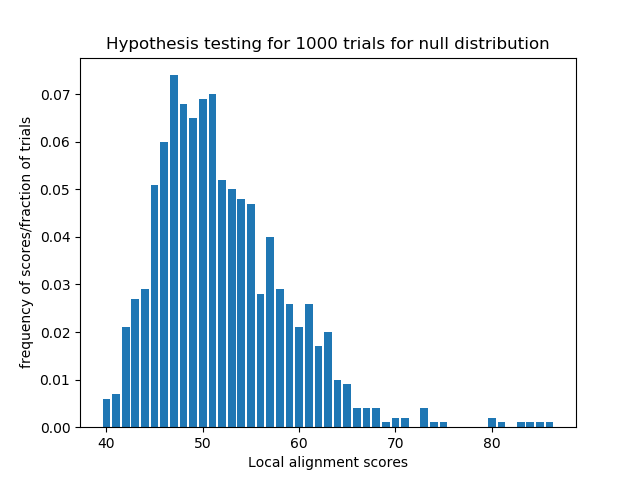
\includegraphics[scale = 1.0, clip=false, trim=0cm 0cm 0cm 0cm]{Q4_bar_graph.png}
\end{figure}
\FloatBarrier

\section*{Answer to Question 5}
\begin{itemize}
    \item mean of the distrubution:  52.0
    \item standard deviation of distribution:  6.72
    \item z-score of the distribution:  122.5
\end{itemize}

\section*{Answer to Question 6}
The z-score is around 100 which means it right at the corner of the bell
shaped distribution. 1$\sigma$ from the mean of around 50 is about 7. And
we know that 3$\sigma$ covers about 99\% of bell shape, i.e the 
likelihood of value falling within 3$\sigma$ is high and the probability of
value to fall outside 3$\sigma$ is  about 1\%. The z-score we found tells us that the value of the score we found in Q1 is about 100 standard deviations away from mean (score of 875 is more than $100\sigma + \mu$). We can find the exact probability using the z test for normal distribution which gives us a probability on the order of $10^{-2000}$ (\href{https://www.wolframalpha.com/input/?i=Probability+of+100+standard+deviations}{source}) which is much smaller than the chance of winning a lottery 

\section*{Answer to Question 7}
\begin{itemize}
    \item Let $x = ``ABC"$ and $y = ``"$. Then global alignment will return $x' = ``ABC"$ and $y' = ``---"$ so $|x| = 3$ and $|y| = 0$ and edit distance need 3 substitution operation to substitute $"---"$ to $``ABC"$ and $score(x', y') = |x'| +|y'| - 3 = 0$. Therefore, \textcolor{red}{\texttt{dash\char`_score}}$ = 0$
    
    \item Let $x = ``ABC"$ and $y = ``ABC"$. Then global alignment returns the same strings and edit distance need zero operations. Hence $score(x, y) = |x| + |y| - 0 = 3 + 3 = 6$. Thus \textcolor{red}{\texttt{diag\char`_score}} must be 2 for the score of $x$,$y$ to be 6
    
    \textcolor{red}{\texttt{diag\char`_score}} = 2
    
    \item Let $x = ``ABC"$ and $y = ``ABT"$. Then global alignment returns the same strings with $score(x, y) = score(``C", ``T") + 2\times $\textcolor{red}{\texttt{diag\char`_score}}. Hence edit distance needs substitution of "T" to "C" i.e one operation. Thus we have:
    
    $score("C", ``T") + 2 \times $\textcolor{red}{\texttt{diag\char`_score}} $= |x| + |y| - 1$
    
  \textcolor{red}{\texttt{off\char`_diag\char`_score}} $= 3 + 3 - 1 - 2 * 2 = 1$.
  
\end{itemize}

\section*{Answer to Question 8}
\begin{itemize}
    \item words within 1 edit distance of string "humble":
    
\{"bumble", "humbled", "tumble", "humble", "rumble", "humbler", "humbles", "fumble", "humbly", "jumble", "mumble"\}

\item words within 2 edit distance of string "firefly":

\{"firefly", "tiredly", "freely", "fireclay", "direly", "finely", "firstly", "liefly", "fixedly", "refly", "firmly"\}
\end{itemize}

\newpage
\appendix
\section{Python code used to answer the Application Questions}
\lstinputlisting{alg_application4_solution.py}
\section{All functions for project 4 used in the application}
\lstinputlisting{alg_project4_solution.py}

\end{document}
